\chapter{Functional evaluation of text-mining tools}
\section{Introduction}
Clinical text from Electronic Health Records (EHRs) has been used for
post-marketing surveillance of drug-induced adverse events
\cite{Harpaz2010,Haerian2012,Wang2009,Friedman2009,Liu2013,Platt2012},
detection of drug-drug interactions \cite{Iyer2013,Duke2012},
discovery and validation of clinical phenotypes
\cite{Lyalina2013,Pathak2013,Davis2013}, and detection of
relationships between clinical concepts, such as drug-disease
treatment pairs
\cite{Jung2014,Chen2008,Zhu2013,deBruijn2011,Patrick2010}.  Raw
clinical text arguably provides the most complete picture of the state
of patients at any point in time since much of the structured data in
EHRs, such as administrative codes, are used primarily for purposes
other than communication of key clinical information about patients –
e.g., billing \cite{Poissant2010,BirmanDeych2005,Carroll2012,Xu2013}.
However, clinical text is unstructured data, and basic questions that
are easy to state in plain language are often difficult to reduce to
practice – for example, find all patients who have Peripheral Artery
Disease and who are taking Cilostazol.  A critical first step in the
use of clinical text to address such electronic phenotyping problems
is finding mentions of entities of interest, such as drugs, diseases
or laboratory values in the text \cite{Boland2013,Bauer2013}.  These
may be positive mentions, indicating that the patient has the disease
or is taking the drug, or negated mentions, such as when a condition
is ruled out.  These mentions may then be used to calculate statistics
to directly address the question at hand, or as the basis for
representing patients for use in data mining approaches
\cite{Boland2013,Bauer2013,Cole2013}.

A variety of Natural Language Processing (NLP) systems that address
this goal have already been developed and are in widespread use
\cite{Chen2004,Davolio2010,Savova2010}.  These may be arranged along a
spectrum of complexity, from very simple, fast string matching systems
to more complex systems incorporating sophisticated statistical
learning methods \cite{Nadkarni2011,Deshmukh2009,Meystre2010}.
Simpler systems typically provide a minimal set of information about
the text, such as mentions of entities of interest and their negation
status.  More complex systems often provide much richer information
about the text, such as part of speech tags and parse trees, in
addition to mentions of entities of interest.  However, this comes at
a significant cost in the form of increased computational demands and,
in the case of supervised learning methods, the need for labeled
training text from which to learn.

In this paper, we present a systematic exploration of the tradeoffs
between simple term recognition and advanced NLP methods when applied
to clinical text for a diverse set of use cases.  We used a modified,
standalone workflow based on the NCBO Annotator
\cite{Noy2009,Lependu2012b,Jonquet2010} and REVEAL (Health Fidelity,
Palo Alto CA), to find mentions of entities of interest in 9 million
clinical notes from the Stanford Translational Research Integrated
Database Environment (STRIDE) \cite{Lowe2009}, and investigated
tradeoffs between these two sets of term-mentions when they were used
in several clinical research tasks (Figure 4.1).

\begin{figure}
  \begin{center}
    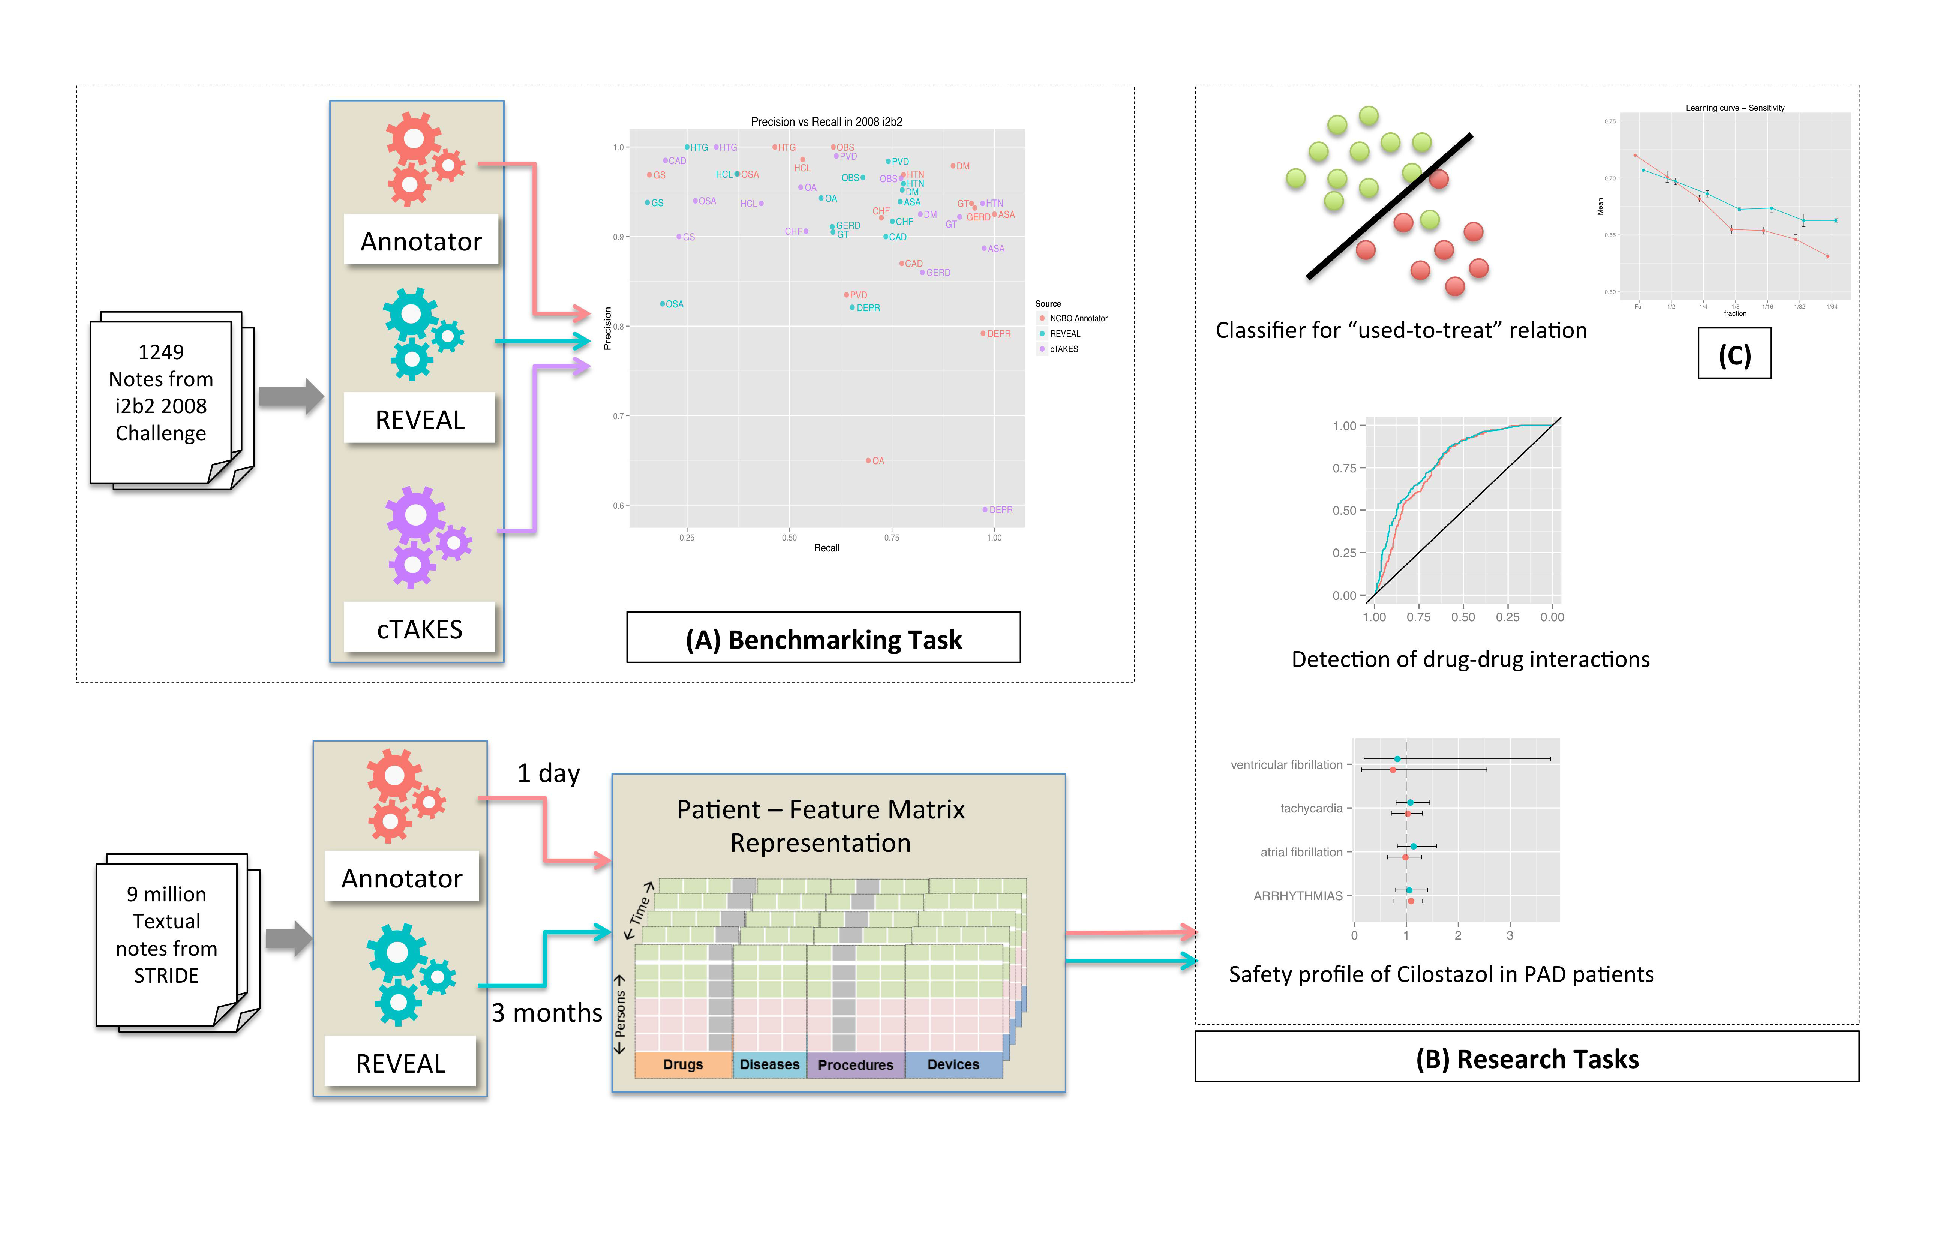
\includegraphics[width=0.9\linewidth]{ch4-figures/Figure1.pdf}
  \end{center}
  \caption[Overview of text processing tool comparison]{Our
    investigation has three parts: (A) First, we benchmark the
    accuracy of the NCBO Annotator based workflow, REVEAL and cTAKES
    on the task of finding mentions of co-morbidities in the 2008 i2b2
    Obesity Challenge dataset (details in Figure 4.2). (B) Second, we
    evaluate the trade-off of using annotations, and the resulting
    patient-feature matrix, from 9 million clinical notes from STRIDE
    generated using the NCBO Annotator based workflow and the REVEAL
    NLP system. The three research tasks are: detection of
    used-to-treat relationships between drugs and indications,
    detection of drug-drug interactions and profiling the safety of
    Cilostazol use in patients with Peripheral Artery Disease. Each of
    these evaluations is based on previously published work; the only
    source of variation is the annotations used as input to the
    published methods. The patient-feature matrix is described in
    detail in Supplemental materials S2. We did not run cTAKES on the
    9 million clinical notes from STRIDE because it would have
    required over a year to complete given our computational
    resources. (C) Finally, we explore the impact of dataset size on
    task of detecting the used-to-treat relation using increasingly
    smaller subsets of the data (details in figure 6).}
  \label{fig:short}
\end{figure}


The NCBO Annotator based workflow is a minimalist system that relies
on a large dictionary of terms, their mappings to UMLS concept IDs
(CUI’s) \cite{Bodenreider2004}, and the NegEx negation detection
system \cite{Chapman2001}, to find mentions of biomedical concepts in
clinical text and establish their negation status.  There is little
“understanding” of the text aside from recognizing a set of words and
phrases, and their negations.  The workflow is deployed quite
directly, using computationally efficient string matching and regular
expression engines \cite{Shah2009,Unitex} that operate directly on the
text without any pre-processing.  In contrast, REVEAL, a commercial
NLP system based on the popular MedLEE system \cite{Friedman2000},
performs various pre-processing steps such as parsing and word sense
disambiguation en route to encoding words and phrases into UMLS codes.
These steps represent a deeper understanding of the structure of the
text than that of the NCBO Annotator based workflow, and are expected
to improve the quality of the annotations.

However, it took roughly 3 months to process our dataset with REVEAL,
while the NCBO Annotator processed the same dataset in a few hours.
It is thus worth exploring what is gained from this extra
computational time when we employ the resulting term-mentions (which
we refer to as annotations) in subsequent tasks.

\section{Materials and Methods}
\subsection{Overview of our approach}
Our investigation has three parts (figure 1).  First, we compared the
accuracy of the NCBO Annotator based workflow and REVEAL on the task
of finding mentions of entities of interest in the 2008 i2b2 Obesity
Challenge dataset \cite{Uzuner2009}, which is a set of discharge notes
manually annotated with the presence/absence of sixteen indications
related to obesity.  This test provides a baseline measurement of the
accuracy of the systems on a task that does not, by itself, count as
direct clinical research.

Second, we compared the NCBO Annotator and REVEAL in three research
tasks that use the resulting annotations in different ways to address
questions of greater clinical significance.  Each of these evaluations
is based on previously published work; the only source of variation is
the annotations used as input to the published methods. In all other
respects, the analyses are identical.  The first task is to profile
adverse events in patients with Peripheral Artery Disease (PAD) who
are taking Cilostazol versus other PAD patients \cite{Leeper2013}.
The second task is to detect adverse drug-drug interactions
\cite{Iyer2014}.  The third task uses mentions of drugs and diseases
to detect used-to-treat relationships between drugs and diseases
\cite{Jung2014}(12).  Finally, we explored the impact of dataset size
on the last of these tasks by repeating the used-to-treat detection
analysis using increasingly smaller random subsets of patients.

\subsection{Data Sources}
We used two sources of clinical text in our evaluations.  First, we
used the manually annotated dataset from the 2008 i2b2 Obesity
Challenge, which consists of 1292 discharge notes that have been
manually annotated by domain experts with the presence/absence of
sixteen indications related to obesity and its comorbidities.  Second,
we used 9 million unstructured clinical notes from the Stanford
Translational Research Integrated Database Environment (STRIDE).
These notes covered approximately 1.2 million patients and 18 years of
data from the Stanford Hospital System and Lucile Packard Children’s
Hospital.

\subsection{Processing clinical text}
The NCBO Annotator finds mentions of biomedical concepts in
unstructured text in two steps.  First, it finds mentions of terms
from a dictionary compiled from 22 clinically relevant ontologies,
such as SNOMED-CT and MedDRA.  We applied a series of syntactic and
semantic suppression rules to the terms from the 22 ontologies to
create a clean lexicon. We keep terms that are predominantly noun
phrases \cite{Xu2010} based on an analysis of over 20 million MEDLINE
abstracts; we remove uninformative phrases based on term frequency
analysis of over 50 million clinical documents from the Mayo clinic
\cite{Wu2012}; and we suppress terms having fewer than four characters
by default because the majority of these tend to be ambiguous
abbreviations.

We then map the terms to UMLS CUIs.  This mapping was tuned on the
STRIDE corpus by identifying ambiguous terms that belong to more than
one semantic group (drug, disease, device, procedure)
\cite{Wu2012,Bodenreider2003} and suppressing their least likely
interpretation. For example “clip” is more likely to be a device than
a drug in clinical text, so we suppress the interpretation as
“Corticotropin-Like Intermediate Lobe Peptide.  Mentions of drugs are
expanded to their ingredients using RxNorm \cite{Nelson2011}.
Finally, NegEx regular expressions are used to flag negative mentions
(e.g., “myocardial infarction was ruled out”) and to determine if a
term is mentioned in the history or family history section of the note
\cite{Chapman2001}.  The result is a list of present, positive
mentions of biomedical concepts, which are about the patient, in the
input text.

In contrast, REVEAL is a commercial text processing system based on
Columbia University’s MedLEE system and developed by Health Fidelity
under an exclusive license \cite{HealthFidelity}.  We obtained a
virtual machine for the REVEAL system under an academic license from
Health Fidelity and used it to process the i2b2 and STRIDE datasets.
Like the NCBO Annotator, REVEAL identifies negated mentions, which are
ignored.  Only positive mentions are used in further analysis.  We
used the same term to concept mapping used by the NCBO Annotator with
REVEAL to assign CUIs.  REVEAL derived annotations thus also benefited
from the tuning of this mapping to the STRIDE dataset.

\subsection{Accuracy on the 2008 i2b2 dataset}
We used the 1249 discharge notes from the 2008 i2b2 Obesity Challenge
to evaluate the accuracy of the systems.  Each note contains ground
truth labels for whether or not each of sixteen indications is
explicitly mentioned in the text.  The ground truth labels are at the
level of entire notes instead of specific locations in each note, so
our evaluation counted any positive mention of the target indications
as indicating the presence of the indication in a given note.  Note
that for this evaluation, we count positive mentions of the
descendants of these CUIs as positive mentions of the listed CUIs, and
this step was performed for all of the evaluated systems.  For this
task, we also evaluated the accuracy of cTAKES version 3.0.0
\cite{Savova2010}, an NLP system specialized for clinical text that
was originally developed at the Mayo Clinic.  We included cTAKES in
this evaluation because it is another widely used clinical
text-processing system and is able to perform approximate matches,
e.g., “joint with pain” is recognized as “joint pain”.  It was not
used further in the functional evaluation because it was
computationally prohibitive – our calculations based on processing the
i2b2 dataset indicated that it would take well over a year to process
all 9 million STRIDE notes, given our computational resources.

\subsection{Safety Profiling of Cilostazol}
Leeper et al \cite{Leeper2013} analyzed the electronic medical records
from the Stanford clinical data warehouse using text-mining to
identify 232 PAD patients taking Cilostazol and a control group of
1,160 patients with PAD but not taking this drug. Over a mean follow
up of 4.2 years, they observed no association between Cilostazol use
and any major adverse cardiovascular event including stroke,
myocardial infarction or death. We used the methods described in
detail in Leeper et al to calculate odds ratios for a set of adverse
events in patients with Peripheral Artery Disease (PAD) who are taking
Cilostazol versus those who are not taking Cilostazol.  Mentions of
clinical concepts in clinical notes from STRIDE are used to build the
case (PAD and Cilostazol) and control (PAD only) cohorts as described
in \cite{Patrick2010}, and to match them for potential confounders.
The odds ratios are based on the positive mentions of the adverse
events in each group.  In this analysis, we compare the odds ratios
and confidence intervals obtained from annotations output from the
NCBO Annotator based workflow and REVEAL.  For this evaluation, we
used the 2-hop ontological expansion, described in \cite{Lependu2013}
and in Supplementary Materials S1, to generate sets of recognized CUIs
for each adverse event, and these were used for all systems.

\subsection{Adverse Drug-Drug Interactions}
Iyer et al \cite{Iyer2014} used mentions of drug and event concepts
from clinical notes to identify drug-drug interactions (DDIs) leading
to adverse events among 1165 drugs and 14 adverse events.  Positive
mentions of drugs and adverse events were used to create timelines of
mentions for each patient, and these were used to calculate adjusted
odds ratios for the drug-drug-event associations.  They validated the
results on a gold standard of 1698 DDIs curated from existing
knowledge bases.

In this study, we detected adverse drug-drug interactions using
mentions of drugs and adverse events in clinical notes from STRIDE,
using methods described in detail in Iyer et al.  Accuracy was tested
on a gold standard set of known drug-drug interactions that was
assembled in Iyer et al from Drugbank \cite{Knox2011} and the
Medi-Span Drug Therapy Monitoring System (Wolters Kluwer Health,
Indianapolis, Indiana, USA).

The output of the NCBO Annotator based workflow and REVEAL on the
STRIDE dataset was used to calculate odds ratios and confidence
intervals for the drug-drug-adverse event triplets in the gold
standard, and receiver-operator characteristic (ROC) curves were
calculated using thresholds on the odds ratios.  As in the Cilostazol
study described above, we used the 2-hop ontological expansion to
generate sets of recognized CUIs for each adverse event.  We compare
the ROC curves derived from the NCBO Annotator and the ROC curves
derived from REVEAL using the method of DeLong et al
\cite{Delong1988}.

\subsection{Learning used-to-treat relationships from clinical text}
Jung et al \cite{Jung2014} described a data-mining approach for
identifying off-label usages using features derived from free text
clinical notes and features extracted from two databases on known
usage (Medi-Span and DrugBank). In that effort, we trained a highly
accurate predictive model to detect novel “used-to-treat”
relationships among 1,602 unique drugs and 1,472 unique
indications. We validated 403 predicted uses across independent data
sources and prioritized them based on drug safety and cost.

We evaluated the utility of mentions of biomedical concepts found by
the NCBO Annotator based workflow and REVEAL respectively in detecting
used-to-treat relationships between drugs and indications, using
methods described in detail in Jung et al. We followed these methods
exactly, except that we used only input features derived from clinical
text.  This is because we are principally interested in the difference
in the predictive value of annotations from the NCBO Annotator based
workflow and REVEAL.

As described in \cite{Platt2012}, a gold standard of positive and
negative examples of used-to-treat relationships compiled from
Medi-Span (Wolters Kluwer Health®, Indianapolis, IN), was split
randomly 4:1 into training and test sets.  Features calculated from
mentions of drugs and indications in the data were used as inputs to
SVM classifiers.  The resulting classifiers were tested on the hold
out test sets.  We used the e1071 library in R to fit the models,
setting the misclassification cost hyperparameter for the SVMs using
10-fold cross validation in the training set.

\subsection{Learning used-to-treat relationships with limited data}
Intuitively, a smaller dataset will have less information about rare
associations.  In those circumstances, analysis may benefit from more
advanced NLP than using simpler methods.  We assessed the impact of
dataset size on the learning task described above.  To create the
reduced datasets, we sampled subsets of patients without replacement
from the whole population of patients in our STRIDE dataset.  The
reduced datasets were of relative size 1/2, 1/4, 1/8, 1/16, 1/32, and
1/64 to the original dataset.  We repeated this sampling process ten
times for each sample size.  For each sample, we used the mentions of
drugs and indications found by either the NCBO Annotator based
workflow or REVEAL to construct features for SVM classifiers as
before.  A classifier was trained and evaluated on a held out test set
for each sample as before.

\section{Results}
\subsection{Accuracy of annotations using the 2008 i2b2 Obesity Challenge}
Figure 4.2 summarizes the precision and recall of the NCBO Annotator,
REVEAL and cTAKES on the 2008 i2b2 Obesity Challenge dataset.
Precision and recall is shown for each indication with the exception
of “venous insufficiency”, for which REVEAL was not able to detect any
mentions.  All systems achieve high precision, but there is
considerable variation in recall, and no system is best across all
indications with respect to either precision or recall.  Overall,
indications that are difficult to detect for one system (e.g.,
gallstones) are difficult for all systems.

\begin{figure}
  \begin{center}
    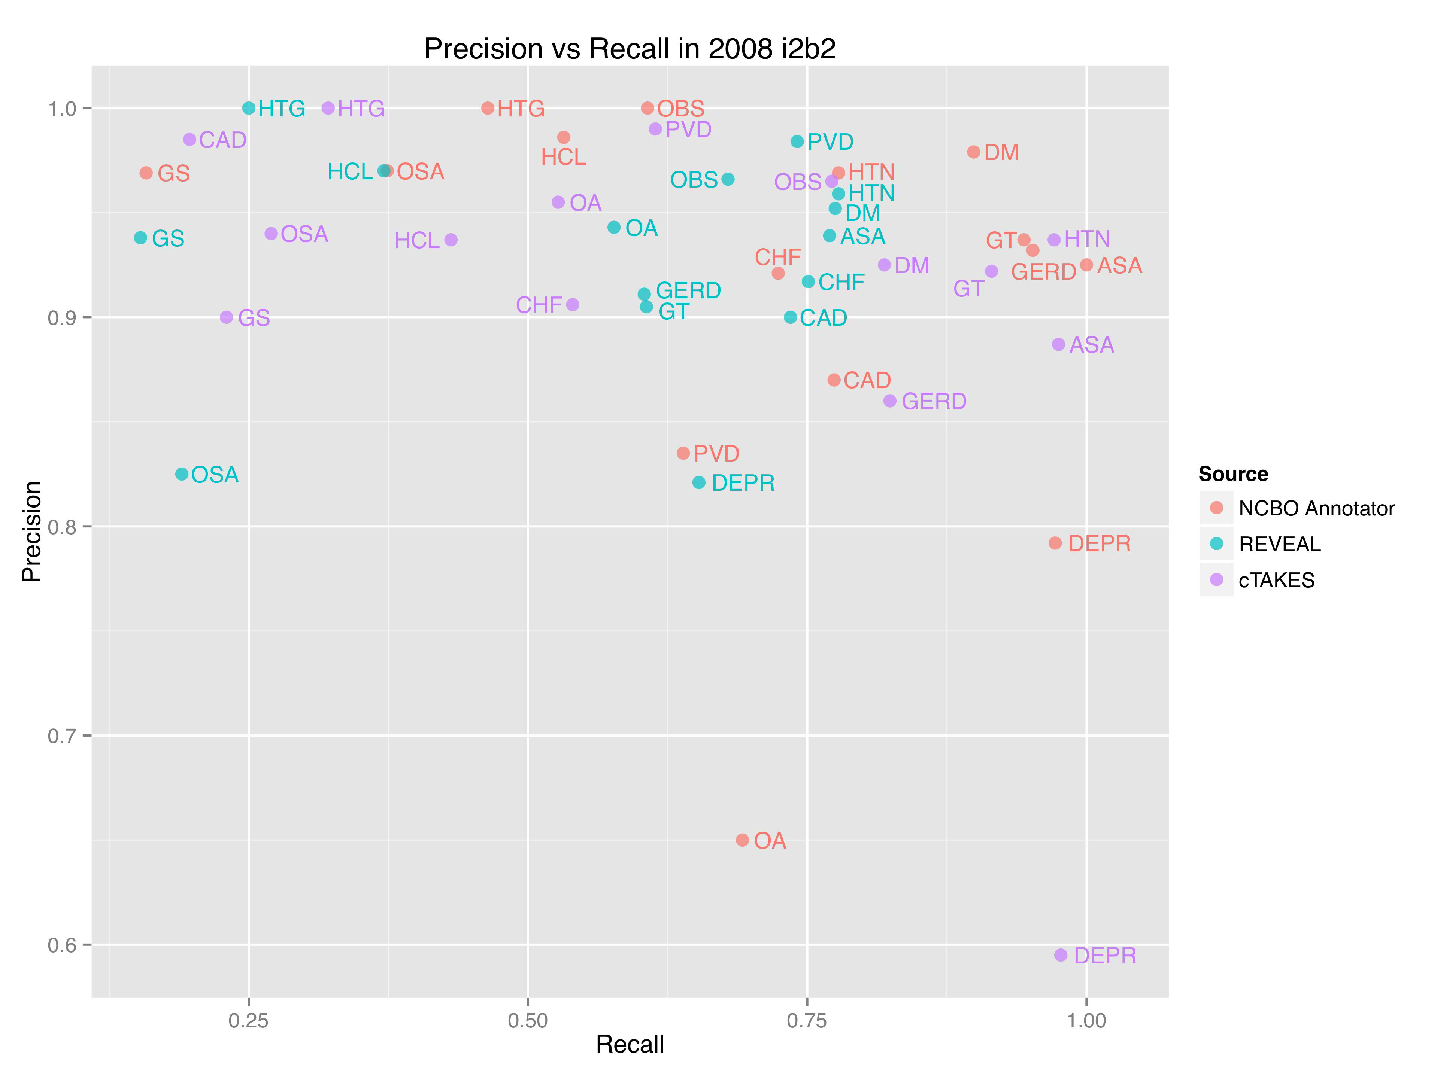
\includegraphics[width=0.9\linewidth]{ch4-figures/Figure2.pdf}
  \end{center}
  \caption[Performance of text processing methods in 2008 i2b2
    Challenge]{The precision and recall of the NCBO Annotator, REVEAL
    and cTAKES in the 2008 i2b2 dataset is plotted here for each
    indication.  There is considerable variation in recall across both
    systems and indications, but generally indications that are hard
    to detect are hard to detect for all systems (e.g., Gallstones –
    labeled here as GS).  There is no universally best system across
    all indications with respect to either precision or recall.
    Labels: ASA=asthma, CAD=coronary artery disease, CHF=congestive
    heart failure, DM=diabetes, DEPR=depression, GS=gallstones,
    GERD=gastro-esophageal reflux disease, GT=gout,
    HCL=hypercholesterolemia, HTN=hypertension,
    HTG=hypertriglyceridemia, OA=osteoarthritis, OBS=obesity,
    OSA=obstructive sleep apnea, PVD=peripheral vascular disease. }
  \label{fig:short}
\end{figure}


\subsection{Safety profiling of Cilostazol}
The goal of this task is to profile adverse events associated with the
use of Cilostazol in patients with Peripheral Arterial Disease.  The
output is odds ratios and confidence intervals for each adverse event.
Figure 4.3 shows results from Leeper et al, which were obtained using
the NCBO Annotator based workflow, along with results from the same
analysis performed using annotations from REVEAL.  There is no
significant difference in either the odds ratios or confidence
intervals for any of the adverse events except for the event ‘sudden
cardiac death’, for which REVEAL found no instances in the data.

\begin{figure}
  \begin{center}
    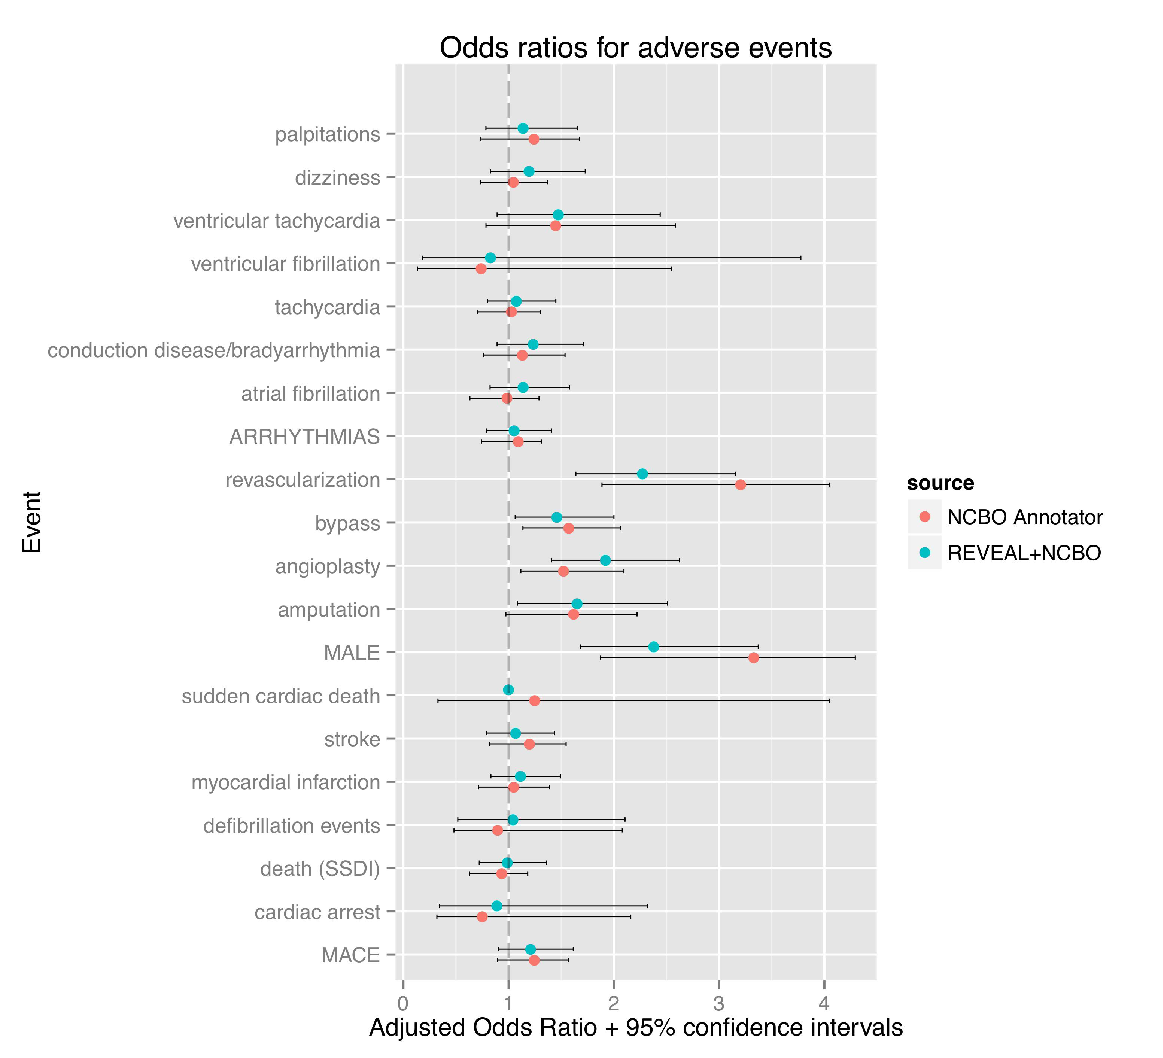
\includegraphics[width=0.9\linewidth]{ch4-figures/Figure3.pdf}
  \end{center}
  \caption[Adverse events in PAD with and without Cilostazol]{Profile
    of adverse events in PAD patients with and without exposure to
    Cilostazol.  The plot shows odds ratios and 95\% confidence
    intervals calculated using annotations from STRIDE using the NCBO
    Annotator based workflow and REVEAL.  There is no change in the
    conclusions of this analysis depending on the text processing
    system being used.  Note that REVEAL did not find any instances of
    “sudden cardiac death” in the data; for this event, we set the
    odds ratio to 1.  }
  \label{fig:short}
\end{figure}


\subsection{Learning adverse drug-drug interactions}
The goal of this task is to use mentions of drugs and indications in
clinical notes from STRIDE to detect adverse drug-drug interactions
following the method of Iyer et al.  The output is a set of adjusted
odds ratios for a gold standard set of known and negative drug-drug
interactions and associated adverse events.  Figure 4.4a shows
Receiver Operator Characteristic (ROC) curves for the gold standard as
we vary the odds ratio threshold for signaling an adverse drug-drug
interaction.  There is no significant difference in the ROC curves
(p-value = 0.275). Figure 4.4b shows the area under the Area Under the
ROC Curve (AUC) for each of 9 adverse events separately.  For all
adverse events, there is no significant difference in the AUC between
the two systems.  Note that this analysis excludes the adverse event,
“serotonin syndrome”, for which the NCBO Annotator is significantly
better than REVEAL (p-value < 1e-6).

\begin{figure}
  \begin{center}
    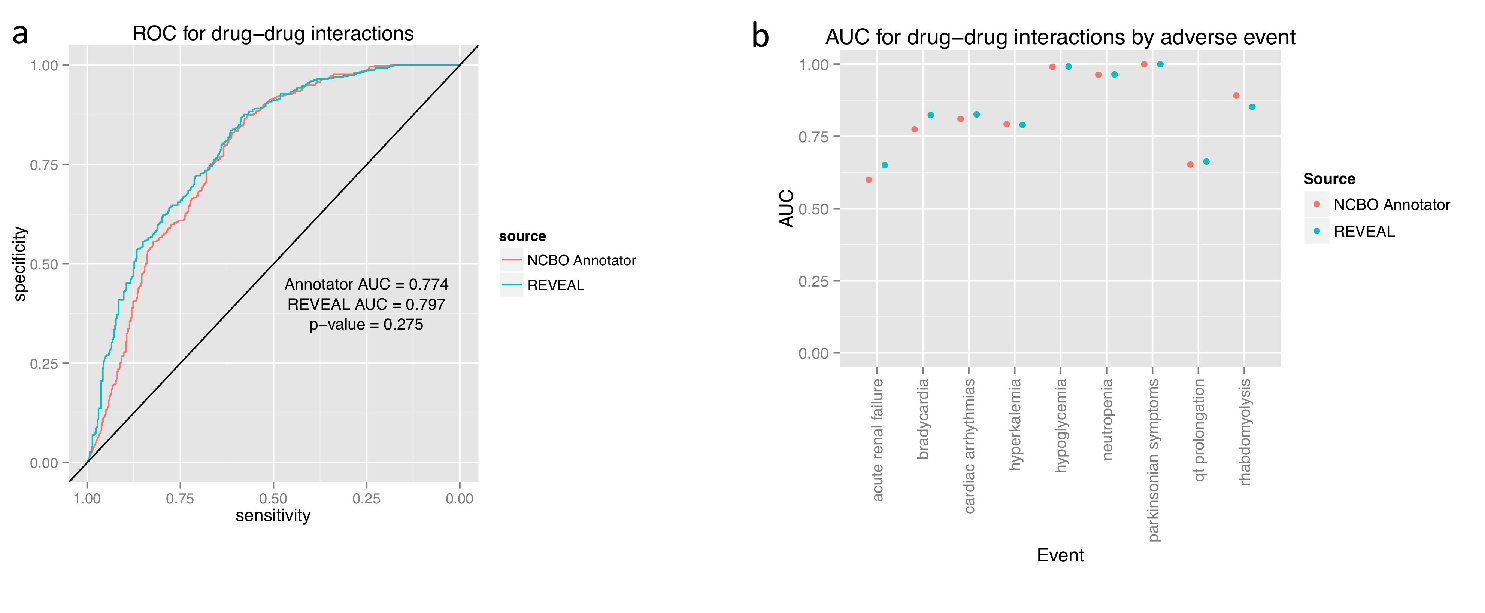
\includegraphics[width=0.9\linewidth]{ch4-figures/Figure4.pdf}
  \end{center}
  \caption[Detection of adverse drug-drug interactions]{Detection of
    adverse drug-drug interactions.  The analysis of Iyer et al was
    carried out using either the NCBO Annotator based workflow or
    REVEAL to process clinical notes from STRIDE.  (a) There is no
    significant difference in the ROC curves (p-value = 0.275 by
    DeLong’s test) for the two systems.  (b) AUCs for each of 9
    adverse events separately.  For all adverse events, there is no
    significant difference in performance (p-values > 0.05).}
  \label{fig:short}
\end{figure}


\subsection{Learning used-to-treat relationships}
The goal of this task is to use mentions of drugs and indications in
clinical notes from STRIDE to construct features that are useful for
identifying which drugs are being used to treat which indications,
according to the methods in Jung et al.  The output is a set of
performance metrics for an SVM classifier, including positive
predictive value, specificity, sensitivity, and F1 based on a hold out
test set. Figure 4.5 shows the performance of classifiers trained and
tested using features derived from the NCBO Annotator based workflow
and REVEAL), and shows that there is no significant difference in
performance (p-value = 0.29 by McNemar’s test).

\begin{figure}
  \begin{center}
    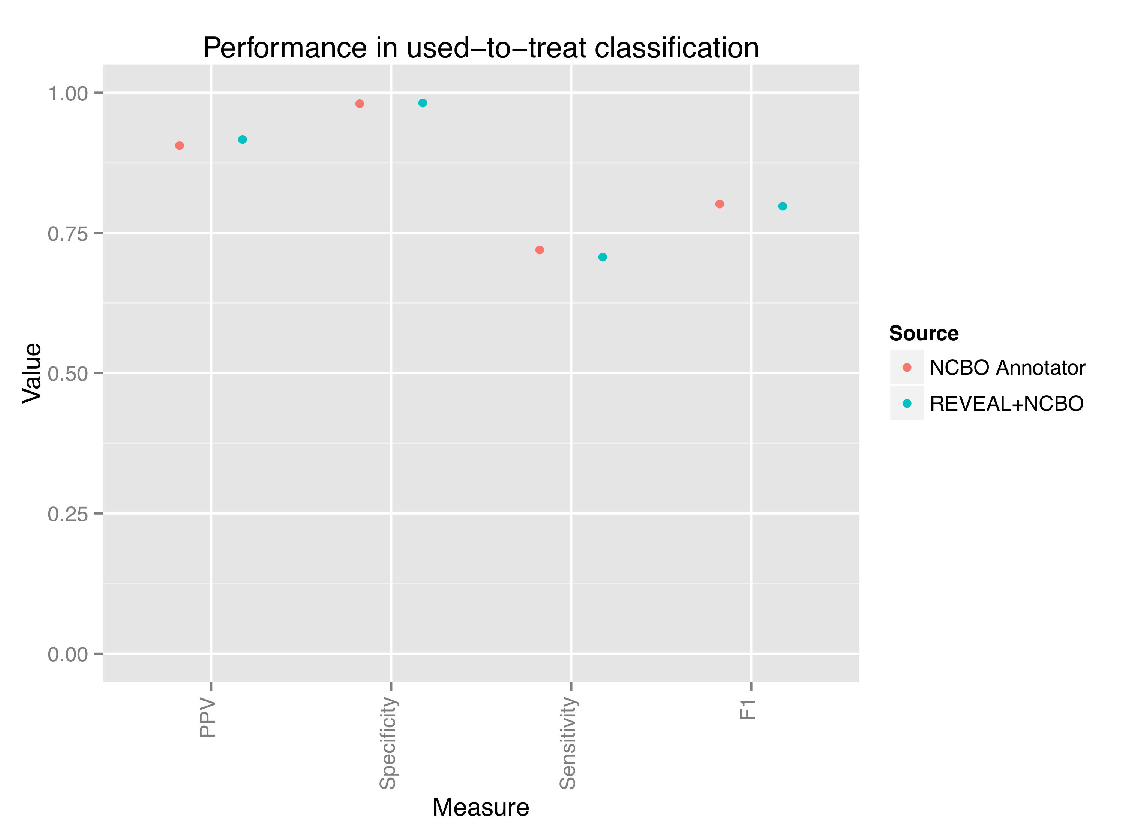
\includegraphics[width=0.9\linewidth]{ch4-figures/Figure5.pdf}
  \end{center}
  \caption[Detecting used-to-treat relationships]{Detecting
    used-to-treat relationships.  We carried out the analysis
    described in Jung et al using either the NCBO Annotator or REVEAL
    to annotate clinical notes from STRIDE.  There is no significant
    difference in performance between classifiers trained and tested
    using features derived from either (p-value = 0.29 by McNemar’s
    Test).}
  \label{fig:short}
\end{figure}


\subsection{Learning used-to-treat relationships with limited data}
We explored whether or not more advanced NLP methods, as embodied in
REVEAL, are advantageous when data is limited so that rare
associations are less well represented in the data.  Figure 4.6 shows
the relationship between dataset size and accuracy of the classifiers
in the used-to-treat task.  Each plot shows the mean performance and
standard error of the mean over ten random samples of patients.  The
gap in accuracy as the dataset size decreases remains quite modest,
even at only 1/64th of the dataset size.  However, the classifiers
trained on output from REVEAL consistently show higher sensitivity
with smaller datasets starting at datasets ¼ the size of the full
dataset.  This ¼ size corresponds to roughly 2.25 million notes, which
would correspond to approximately 250,000 patients if each patient had
the median number of notes. These results agree with the notion that
more advanced NLP will be advantageous when detecting rare
associations or when data is limited.

\begin{figure}
  \begin{center}
    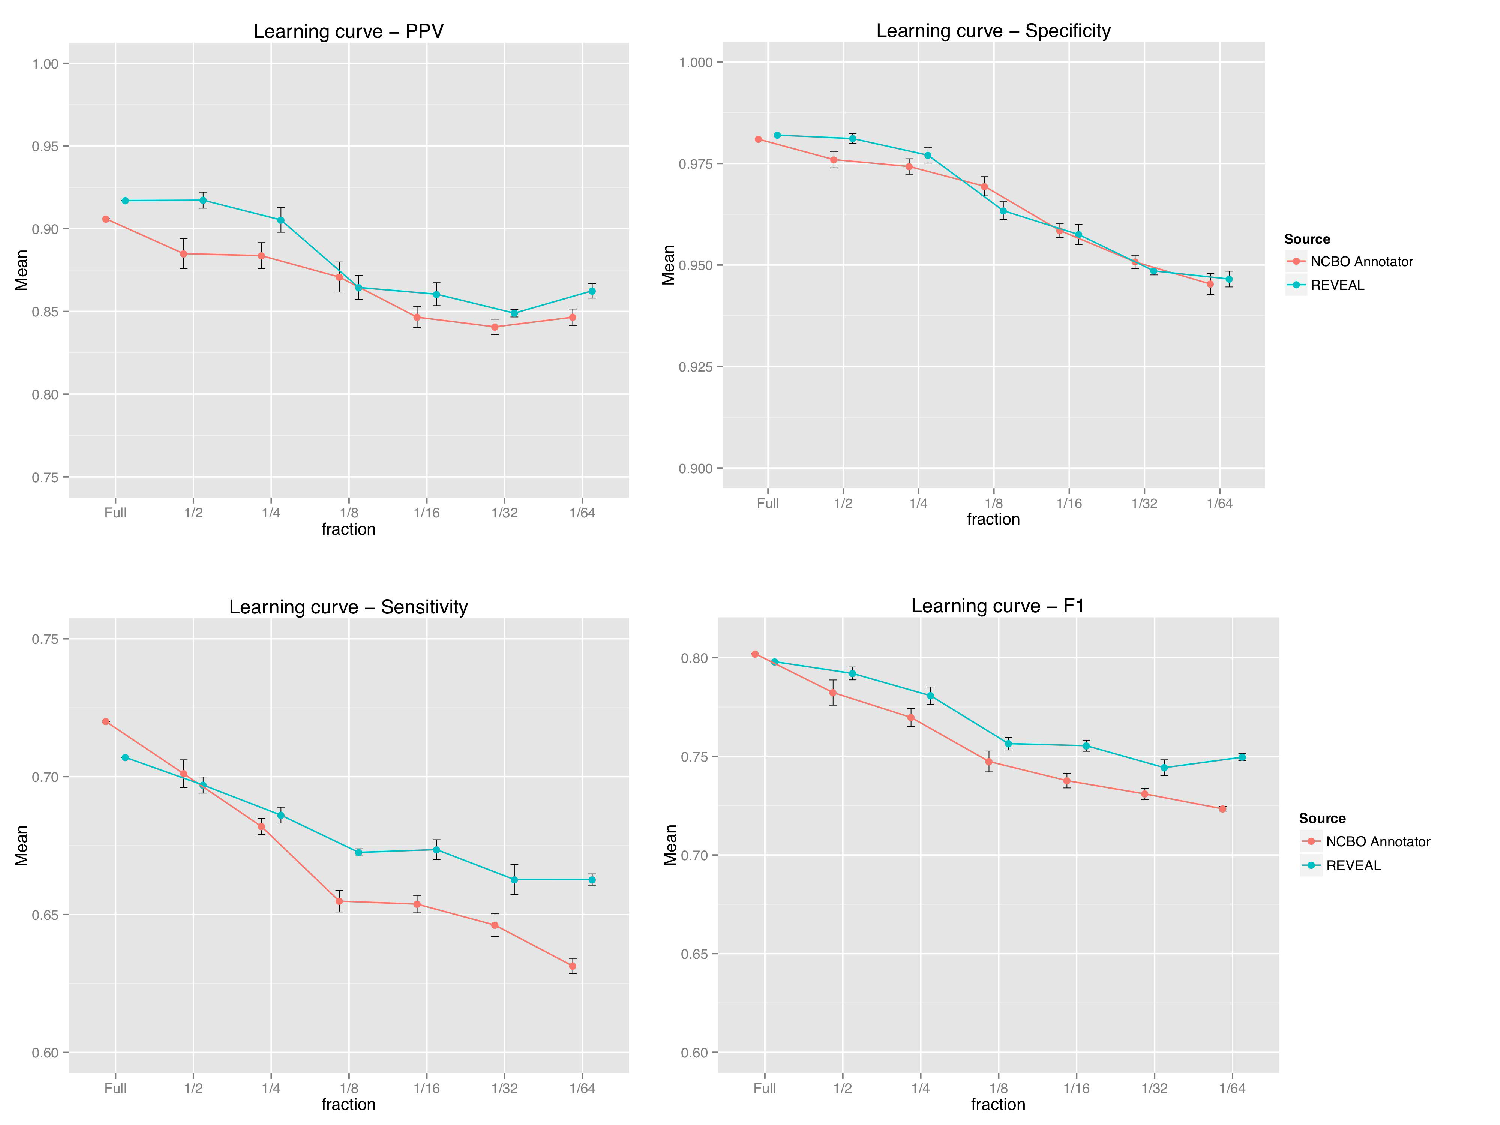
\includegraphics[width=0.9\linewidth]{ch4-figures/Figure6.pdf}
  \end{center}
  \caption[Learning used-to-treat relationships with limited
    data]{Learning curves for the used-to-treat task. We sampled
    random subsets of patients and used the associated notes to
    generate features based on the annotations of those notes by
    either the NCBO Annotator or REVEAL.  This was repeated 10 times
    for each fraction of the full STRIDE dataset.  The mean
    performance metric across the 10 runs is plotted, along with the
    standard error of the mean.  REVEAL has higher sensitivity in
    smaller datasets, and generally has higher precision/PPV.}
  \label{fig:short}
\end{figure}


\section{Discussion}
Recognizing mentions of drugs and diseases in clinical text is a key
step in using the unstructured text from EHRs to address many
questions of clinical interest.  In this paper, we have performed a
systematic comparison of the tradeoff between simple term recognition
and the deeper linguistic understanding of clinical text provided by
advanced NLP, as embodied by the NCBO Annotator and REVEAL
respectively.  The NCBO Annotator uses mgrep and an extensive
dictionary mapping strings to biomedical concepts, along with the
NegEx negation detection module, to efficiently find mentions of the
concepts in text.  In contrast, REVEAL performs extensive
preprocessing, including parsing, word sense disambiguation, and other
core NLP tasks en route to identifying mentions of drugs and diseases.
It is significantly more computationally expensive than the NCBO
Annotator based workflow. For example, the average time to process one
clinical note using REVEAL is 10 seconds, whereas with the NCBO
Annotator based workflow it is 0.01 seconds.  Furthermore, the NCBO
Annotator is a freely available tool while REVEAL is a commercial
product.  These tools were evaluated on a set of clinical research
tasks – safety profiling of Cilostazol, learning adverse drug-drug
interactions, and learning used-to-treat relationships between drugs
and diseases.  We also evaluated the accuracy of the systems in
finding positive mentions of 16 diseases in a manually annotated set
of clinical notes from i2b2.  We found little difference in accuracy
between the methods in any of the three clinical research tasks.

The clinical research tasks we undertook used aggregate statistics
over an entire corpus of clinical text.  In such tasks, all that
matters is that we accurately count mentions of drugs and indications
in the text.  We note that the best performing systems in the textual
portion of the 2008 i2b2 Obesity Challenge were similar in spirit to
the NCBO Annotator \cite{Uzuner2009}.  In the summary paper on that
challenge \cite{Uzuner2011}, Uzuner writes, “Most of the factual and
objective pieces of information were identified by simple rule-based
systems armed with dictionaries of terms and negation extraction
modules”.  Our findings mirror that viewpoint and it seems that for
the set problems we examined, having a good negation detection module,
a comprehensive dictionary, and a best-effort mapping of strings to
concepts are the key ingredients necessary for excellent accuracy.
More advanced NLP techniques do not appear to add much value to such
tasks, and take a much longer time to run.  We note that using REVEAL
to find strings of interest, and then using our mapping of strings to
concepts consistently performed better at the i2b2 annotation task
than the default mapping provided by REVEAL itself.  This suggests
that the quality of the mapping of strings to concepts is one of the
key differences between the systems.  In work evaluating extensions of
cTAKES for document classification, Garla et al found that much of
their tuning consisted of adding terms and lexical variants of terms
to their dictionary \cite{Garla2011}.

These results do not mean that the simple approach embodied by
dictionary based approaches, such as the NCBO Annotator, is
necessarily best for all problems.  For instance, the used-to-treat
task is formulated as a population level problem instead of asking
whether a drug is being used to treat a disease as asserted in a
particular note.  For the latter type of question, in which we want to
infer complex relationships between entities within a given text, the
richer linguistic information output by a full NLP system, such as
part of speech tags, a dependency parse, etc, can be very useful
\cite{Goldstein2009}.  Furthermore, we found that features derived
from REVEAL were more predictive of the used-to-treat relationship
than features derived from the NCBO Annotator based workflow as we
decreased the size of the dataset.  This is consistent with the
intuition that as the dataset size decreases, rare associations may be
more difficult to detect using simple text processing methods.  Thus,
it may be worthwhile to use a full-featured system when the dataset is
relatively small.  It should also be noted that while the upfront
computational cost of running REVEAL on a large corpus may appear
large, it is a one-time cost.  And finally, we note that the systems
were used “out of the box” (i.e., without any special tuning for the
evaluation tasks).  Given that the analysis methods were originally
developed for dictionary-based approaches they could be more effective
in using that output.  It is certainly possible that different methods
that take explicit advantage of the richer information provided by
more advanced NLP methods could outperform the original
methods. However the gain would come at a significant computational
cost, and require expertise that currently only exists in specialized
NLP research teams.

These caveats notwithstanding, our results suggest that for a variety
of questions of clinical interest, it is feasible to use very simple
and fast approaches in lieu of more complex approaches in deriving
useful information from the unstructured data in EHRs.

\section{Conclusion}
Widespread adoption of EHRs is creating a new source of data as a
by-product of routine clinical care.  This data is increasingly
recognized as an asset that can be used to address problems in public
health, health care economics, quality of care, drug safety
surveillance, and even personalized medicine
\cite{Pathak2013,Pathak2013b,Denny2013,Jensen2012,Murdoch2013,Murff2011,Shah2013}.
However, extracting actionable information from EHRs is a challenging
problem because much of its value resides in unstructured text.  NLP
has been applied to this problem to good effect.  In this paper, we
have explored the tradeoff between using a free, simple but fast term
recognition system and a more advanced commercial NLP system.  We
evaluated the systems in a variety of tasks that address questions of
clinical interest.  These tasks ranged from canonical studies that use
the mentions of drugs and diseases to calculate odds ratios, such as
assessing the safety profile of a particular drug in a well-defined
patient population, to a machine learning approach to finding
used-to-treat relationships at the population level.  We achieve the
same accuracy in all three clinical research tasks
